\documentclass[11pt]{article}

\usepackage[utf8]{inputenc}
\usepackage{lipsum}
\usepackage[margin=25mm]{geometry}
\usepackage[labelfont=bf, font=small]{caption}
\usepackage{subcaption}
\usepackage{fancyhdr}
\usepackage{graphicx}
\graphicspath{ {./images/} }
\usepackage{multirow}

\usepackage{hyperref}
\hypersetup{
	linktoc=all,
	colorlinks=true,
	linkcolor=black,
	urlcolor=black,
	pdftitle={Relazione Progetto Reti Logiche}
}

% stuff for drawing graphs
\usepackage{tikz}
\usetikzlibrary{automata, positioning, arrows.meta, shadows.blur}
\tikzset{
    node distance=7cm,    % minimum distance between two nodes
    font=\tt,
    every node/.style={
        align=center,
        fill=white,
    },
    every state/.style={    % default style for all states
        very thick,
        draw,
        circle,
        fill=gray!10,         % fill color
        minimum size=2cm,
        blur shadow
    },
    initial/.style={        % style for initial state
        fill=gray!40        % fill color
    },
    double distance=2pt,    % gap between double circles
    every edge/.style={     % default style for all edges
        draw,
        auto,
        thick,
        -{Latex[length=3mm]}
    }
}
\let\epsilon\varepsilon

% format sections
\usepackage{titlesec}
\titleformat{\section}
{\Large\bfseries}{\thesection}{1em}{}
[\titlerule]

\setlength{\parskip}{1mm}
\setlength{\parindent}{0em}
\setlength{\tabcolsep}{2mm}

\renewcommand*\contentsname{Indice}

\begin{document}

\begin{titlepage}
    
    \vspace*{2cm}
    
    \begin{center}
        \huge{\bfseries Progetto Finale di Reti Logiche} \\[10pt]
        \large{a.a. 2020/2021} \\
    \end{center}
    
    \vfill
    
    \begin{flushleft}
        \large
        \textbf{Alessandra Moro} \\
        \normalsize
        codice persona: 10620673 \\ 
        alessandra.moro@mail.polimi.it \\[5mm]
        
        \large
        \textbf{Alberto Mosconi} \\
        \normalsize
        codice persona: 10653349 \\
        albertomaria.mosconi@mail.polimi.it
    \end{flushleft}
    
\end{titlepage}

\thispagestyle{empty}
\tableofcontents
\newpage

\setcounter{page}{1}
\section{Introduzione}

    \subsection{La specifica del problema}

    Lo scopo del progetto è la realizzazione di un componente hardware per svolgere l'equalizzazione dell'istogramma di una immagine in scala di grigi.
    
    Questa tecnica permette di manipolare i livelli di grigi dei pixel di una data immagine in modo da incrementarne il contrasto. La figura 1 illustra il prima e il dopo di questo processo.
    
    \begin{figure}[h]
        \centering
        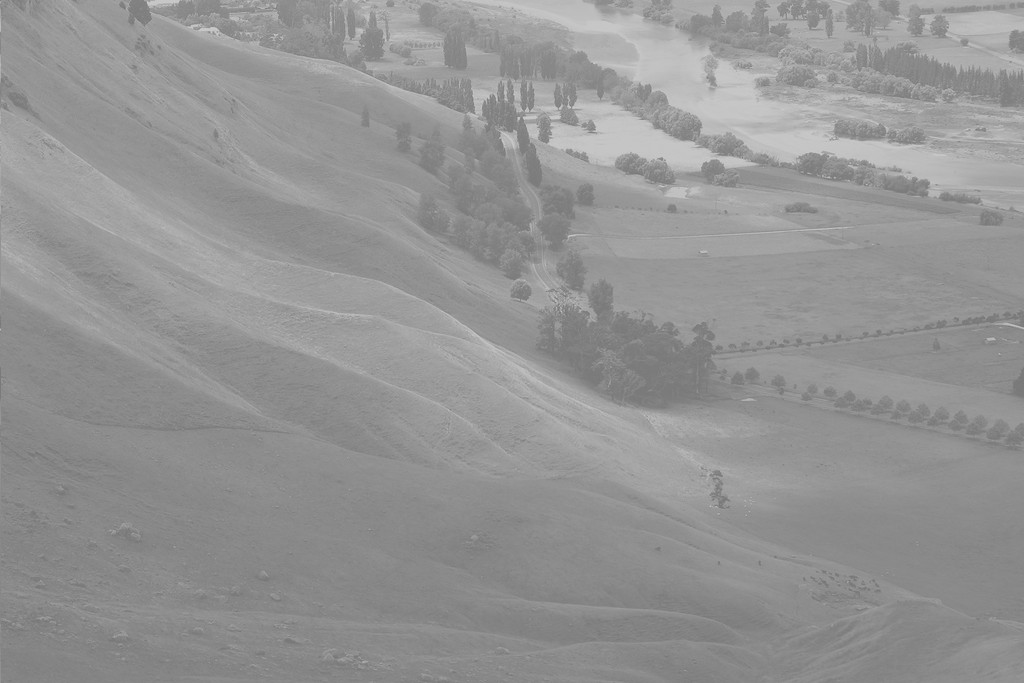
\includegraphics[width=0.4\textwidth]{before-eq.jpg}
        \qquad
        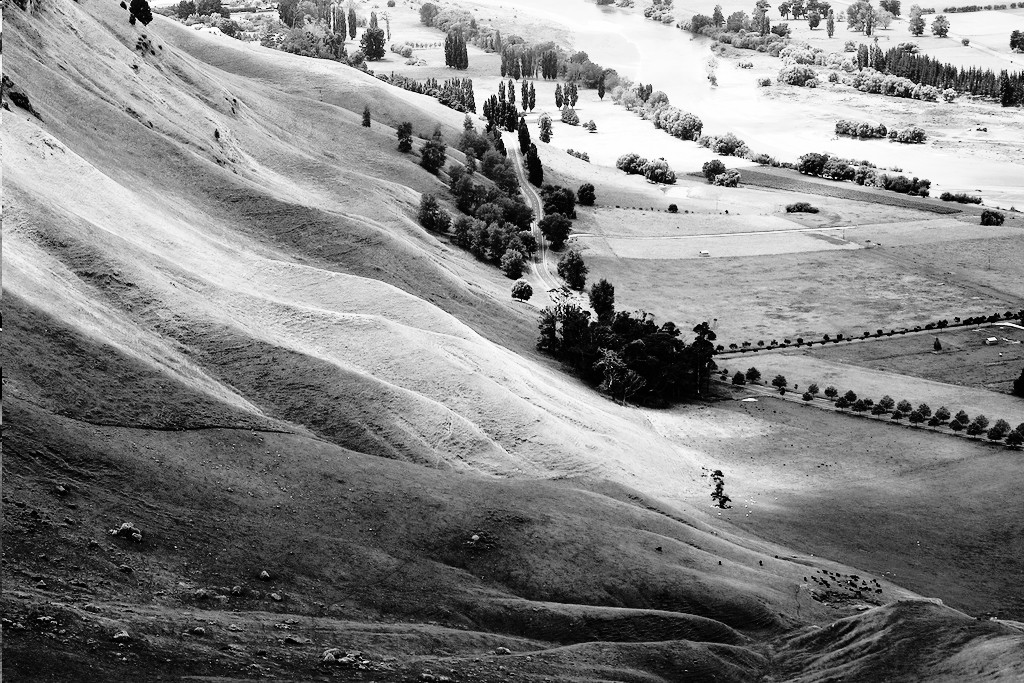
\includegraphics[width=0.4\textwidth]{after-eq.jpg}
        \caption{Confronto prima (sinistra) e dopo (destra) l'equalizzazione [wikipedia]}
    \end{figure}
    
	Il componente sviluppato si interfaccia con una memoria RAM, con indirizzi di 16 bit e celle da 8 bit, da cui legge prima le due dimensioni dell'immagine, e poi sequenzialmente tutti i valori dei pixel.

	Sempre sulla RAM, dopo aver concluso l'elaborazione, scrive i nuovi valori dei pixel. 

\renewcommand{\arraystretch}{1.2}
\begin{center}
        \begin{tabular}{c|c|l}
		\texttt{INDIRIZZO} & \texttt{VALORE} & \tt NOTE \\
            	\hline
		0 & 4 & \tt numero di colonne \\
		1 & 4 & \tt numero di righe \\
		2 & 138 & \tt primo byte immagine \\
		3 & 204 & \\
		4 & 64 &\\
		5 & 64 &\\
		6 & 204 &\\
		7 & 89 &\\
		... & ... & 
	\end{tabular}
\end{center}
\newpage
\subsection{Un esempio di equalizzazione}
    
    Si prende come esempio l'immagine sottostante, di dimensioni 4x4 pixel, e si vuole svolgere il processo di equalizzazione.
    
    \renewcommand{\arraystretch}{1.9}
    \begin{figure}[h]
        \centering
        \begin{subfigure}{0.45\textwidth}
            \centering
            
\includegraphics[width=0.5\textwidth]{example-small.png}
        \end{subfigure}
        \begin{subfigure}{0.45\textwidth}
            \centering
            \begin{tabular}{ |c|c|c|c| }
                \hline
                138 & 204 & 64 & 64\\
                \hline
                204 & 64 & 89 & 64\\
                \hline
                64 & 138 & 89 & 138\\
                \hline
                138 & 204 & 204 & 64\\
                \hline
            \end{tabular}
        \end{subfigure}
        
        \caption{A sinistra l'immagine e a destra i valori dei pixel corrispondenti.}
    
    \end{figure}
    
    Per ricalcolare il valore di ogni pixel bisogna prima trovare il massimo e minimo valore che possono assumere nell'immagine originale, e calcolare la differenza tra i due.\\
    $$\mathtt{
    DELTA\_VALUE = MAX\_PIXEL\_VALUE - MIN\_PIXEL\_VALUE
    }$$
    
    Nel caso dell'esempio si ha che il minimo livello di grigio assunto da un pixel è pari a 64, e dunque \texttt{MIN\_PIXEL\_VALUE=64}, e il massimo è 204, \texttt{MAX\_PIXEL\_VALUE=204}.\\
    Ricavo quindi che \texttt{DELTA\_VALUE=140}.
    
    A questo punto si può ricavare il valore \texttt{SHIFT\_LEVEL}, che serve per gli step successivi.\\
    $$\mathtt{
    SHIFT\_LEVEL = (8 - floor(log_2(DELT\_VALUE + 1)))
    }$$
    
    Nel caso dell'esempio:\\
    $$\mathtt{
    SHIFT\_LEVEL = (8 - floor(log_2(141))) = (8 - floor(7.139)) = (8 - 7) = 1
    }$$
    
    Ora, per ognuno dei pixel che compongono l'immagine, si trova il nuovo valore temporaneo:\\
    $$\mathtt{
    TEMP\_PIXEL = (CURRENT\_PIXEL\_VALUE - MIN\_PIXEL\_VALUE) << SHIFT\_LEVEL
    }$$
    
    E si salva il nuovo valore limitandolo ad un massimo di 255:\\
    $$\mathtt{
    NEW\_PIXEL\_VALUE = min(255, TEMP\_PIXEL)
    }$$
    
    La seguente tabella mostra questi calcoli applicati a tutta l'immagine.
    
    \renewcommand{\arraystretch}{1.2}
    \begin{center}
        \begin{tabular}{c|c|c}
            \texttt{CURRENT\_PIXEL\_VALUE} & \texttt{TEMP\_PIXEL} & \texttt{NEW\_PIXEL\_VALUE} \\
            \hline
            138 & 148 & 148 \\
            204 & 280 & 255 \\
            64 & 0 & 0 \\
            64 & 0 & 0 \\
            204 & 280 & 255\\
            64 & 0 & 0 \\
            89 & 50 & 50 \\
            64 & 0 & 0 \\
            64 & 0 & 0 \\
            138 & 148 & 148 \\
            89 & 50 & 50 \\
            138 & 148 & 148 \\
            138 & 148 & 148 \\
            204 & 280 & 255 \\
            204 & 280 & 255 \\
            64 & 0 & 0 \\
        \end{tabular}
    \end{center}
    
    \vspace{10mm} 
    Sono stati ottenuti così tutti i nuovi valori dei pixel, e l'immagine è stata equalizzata.
    \renewcommand{\arraystretch}{1.9}
    \begin{figure}[ht]
        \centering
        \begin{subfigure}{0.32\textwidth}
            \centering
            
\includegraphics[width=0.7\textwidth]{example-small.png}
        \end{subfigure}
        \begin{subfigure}{0.32\textwidth}
            \centering
            
\includegraphics[width=0.7\textwidth]{example-small-eq.png}
        \end{subfigure}
        \begin{subfigure}{0.32\textwidth}
            \centering
            \begin{tabular}{ |c|c|c|c| }
                \hline
                148 & 255 & 0 & 0 \\
                \hline
                255 & 0 & 50 & 0 \\
                \hline
                0 & 148 & 50 & 148 \\
                \hline
                148 & 255 & 255 & 0 \\
                \hline
            \end{tabular}
        \end{subfigure}
        
        \caption{In ordine, l'immagine originale, l'immagine equalizzata e i valori dei suoi pixel corrispondenti.}
    
    \end{figure}
\newpage
\section{Architettura}
    Il processo di equalizzazione si divide in due fasi: 
    \begin{itemize}
        \item una prima fase in cui vengono cercati e riconosciuti il valore massimo ed il valore minimo tra i pixel costituenti l'immagine ed infine calcolato lo shift level, 
        \item una seconda fase in cui, ripartendo dall'indirizzo contenente il primo byte, vengono calcolati i valori dei nuovi pixel e scritti nelle celle di memoria della RAM.
    \end{itemize}
    
    Il modulo implementato si comporta come una Macchina a Stati Finiti (FSM).

    \subsection{La macchina a stati finiti}
    
        \begin{figure}[h]
            \centering
            \resizebox{\linewidth}{!}{%
            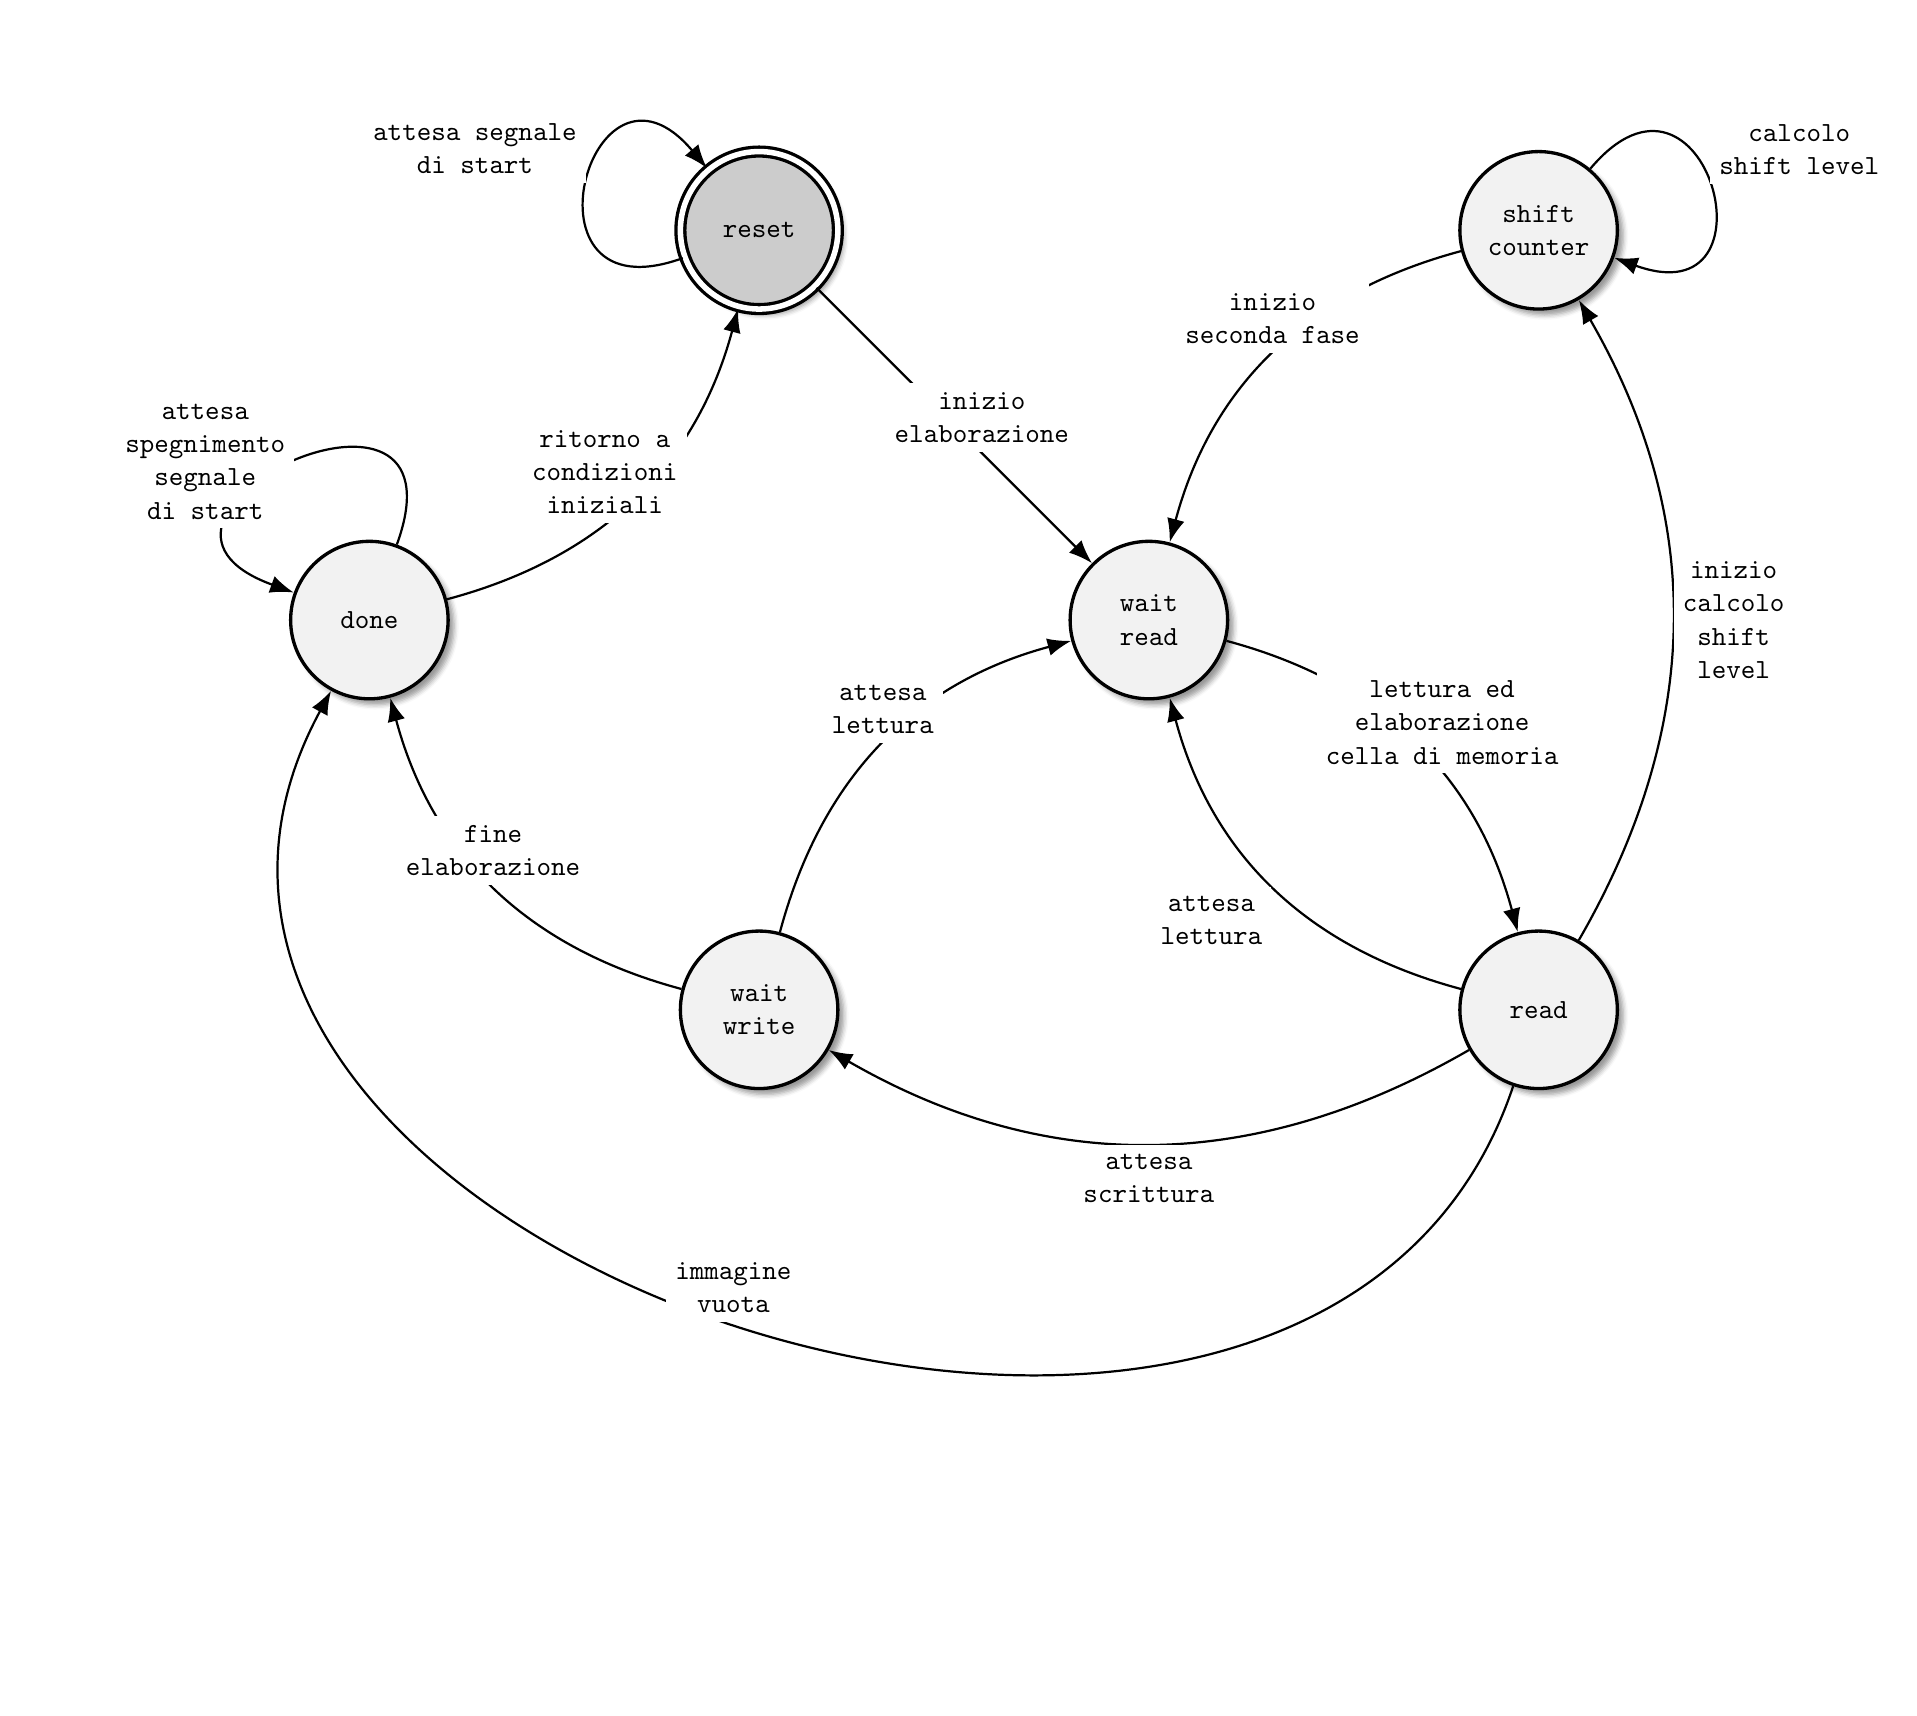
\begin{tikzpicture}
                \node[state, initial, accepting] (s0) {reset};
                \node[state, below right of=s0] (s1) {wait\\read};
                \node[state, below right of=s1] (s2) {read};
                \node[state, above right of=s1] (s3) {shift\\counter};
                \node[state, below left of=s1] (s4) {wait\\write};
                \node[state, below left of=s0] (s5) {done};
                \draw (s0) edge [loop, out=200, in=130, looseness=5] node {attesa segnale\\di start} (s0);
                \draw (s0) edge node[above, pos=0.6] {inizio\\elaborazione} (s1);
                \draw (s1) edge [bend left] node[above, pos=0.6] {lettura ed\\elaborazione\\cella di memoria} (s2);
                \draw (s2) edge [bend left] node {attesa\\lettura} (s1);
                \draw (s2) edge [bend right] node[right] {inizio\\calcolo\\shift\\level}(s3);
                \draw (s3) edge [loop, out=50, in=340, looseness=5] node {calcolo\\shift level} (s3);
                \draw (s3) edge [bend right] node[above] {inizio\\seconda fase} (s1);
                \draw (s2) edge [bend left] node {attesa\\scrittura} (s4);
                \draw (s2) edge [bend left, out=90, in=80, looseness=1.3] node[above] {immagine\\vuota} (s5);
                \draw (s4) edge [bend left] node[above] {attesa\\lettura} (s1);
                \draw (s4) edge [bend left] node[above] {fine\\elaborazione} (s5);
                \draw (s5) edge [loop, out=70, in=160, looseness=5] node[left] {attesa\\spegnimento\\segnale\\di start} (s5);
                \draw (s5) edge [bend right] node[above, pos=0.4] {ritorno a\\condizioni\\iniziali} (s0);
            \end{tikzpicture}%
            }
        \end{figure}
        \subsubsection{Prima fase}
        Partendo dallo stato di \texttt{RESET}, in cui tutti i segnali corrispondono al loro valore di default, si attende che il segnale di start venga portato a 1.
        
        Quando ciò si verifica, sequenzialmente, iniziano la lettura ed il salvataggio delle dimensioni di righe e colonne ed il confronto tra i valori dei pixel per determinarne un massimo ed un minimo. Questo processo avviene con l'alternarsi di due stati.
        \begin{itemize}
            \item Il primo, \texttt{WAIT READ}, ha lo scopo di attendere che la RAM legga il valore richiesto e lo restituisca in output.
            \item Il secondo, \texttt{READ}, invece, riceve in input il valore letto dalla cella di memoria RAM, e si occupa di salvare rispettivamente il numero di colonne, il numero di righe, ed i valori di massimo e di minimo.
        \end{itemize}
        
        Dopo aver stabilito massimo e minimo, avviene il passaggio allo stato \texttt{SHIFT COUNTER}, dove inizia il calcolo del valore di shift (shift level).
        
        Riprendendo la formula per calcolare lo shift level, definita nella specifica dell'algoritmo,
        $$\mathtt{
        SHIFT\_LEVEL = (8 - floor(log_2(DELTA\_VALUE + 1)))
        }$$
        
        si può notare che il sottraendo $\mathtt{floor(log_2(DELTA\_VALUE + 1))}$ equivale al minimo numero di bit necessari per rappresentare $\mathtt{(DELTA\_VALUE + 1)}$.
        
        Pertanto, servendosi di un segnale \texttt{pos\_count} inizializzato al numero massimo di bit (8), si analizza il vettore $\mathtt{(DELTA\_VALUE + 1)}$ partendo dal bit più significativo, ovvero quello in posizione \texttt{pos\_count}, e lo si scorre bit per bit fino a quello meno significativo.
       
        Finché si incontra un bit uguale a 0, \texttt{pos\_count} viene decrementato di 1 e si rimane sullo stato \texttt{SHIFT COUNTER}.
        
        Nell'istante in cui si incontra il bit più significativo pari ad 1, \texttt{pos\_count} non viene ulteriormente decrementato poiché il suo valore corrisponde a quello cercato.
        
        Svolti questi passaggi, si calcola lo shift level e si inizia la seconda fase tornando allo stato di \texttt{WAIT READ}.
        
        \subsubsection{Seconda fase}
        
       Ripartendo dall'indirizzo contenente il primo byte, si inizia un processo analogo alla prima fase, leggendo iterativamente tutti i byte dell'immagine.
        
        Ogni valore letto viene utilizzato nello stato \texttt{READ} per il calcolo del pixel equalizzato, come indicato nella specifica dell'algoritmo.
        
        Ottenuto il nuovo valore, passando attraverso lo stato \texttt{WAIT WRITE}, si attende la scrittura dello stesso nella prima cella di memoria libera, il cui indirizzo si può ricavare facilmente conoscendo le dimensioni dell'immagine. 
        
        Supponendo che il byte letto si trovi ad un indirizzo \texttt{X}, l'indirizzo $\mathtt{X_1}$ di scrittura risulta:
        
        $$\mathtt{X_1= X + (n\_righe \times n\_colonne)}$$
        
        In seguito all'avvenuta scrittura, si torna allo stato \texttt{WAIT READ} per la lettura del successivo byte.
        
        Esauriti tutti i byte dell'immagine, si è concluso il processo di equalizzazione e dallo stato di \texttt{WAIT WRITE} si passa direttamente allo stato \texttt{DONE} portando ad 1 il segnale \texttt{o\_done}.
        
        La permanenza in questo stato termina non appena il segnale di start viene spento; a questo punto si torna nello stato \texttt{RESET} in attesa della prossima immagine.
        
    \subsection{Implementazione in VHDL}
    
    La FSM è implementata con un singolo processo, sensibile agli eventi di clock e di reset. Se il segnale di reset viene portato ad 1 in qualsiasi momento, la macchina è riportata nello stato \texttt{RESET}, riassegnando ad ogni segnale il proprio valore di default.
    
    Sono elencati di seguito i segnali e le variabili utilizzati.
    
    \renewcommand{\arraystretch}{1.1}
    \begin{figure}[h]
        \centering
        \tt
        \begin{tabular}{|p{0.22\textwidth}|p{0.18\textwidth}|p{0.54\textwidth}|}
            \hline
            SEGNALE/VARIABILE & DETTAGLI & FUNZIONE  \\
            \hline
            n\_col & vector, 8bit & Numero di colonne dell'immagine \\
            \hline
            n\_rig & vector, 8bit & Numero di righe dell'immagine \\
            \hline
            current\_address & vector, 16bit & Indirizzo cella in lettura \\
            \hline 
            current\_state & state\_type & Stato corrente della FSM \\
            \hline
            max\_pixel\_value & vector, 8bit & Valore massimo assunto dai pixel dell'immagine \\
            \hline
            min\_pixel\_value & vector, 8bit & Valore minimo assunto dai pixel dell'immagine \\
            \hline
            shift\_level & vector, 4bit & Numero di posizioni di shift, usato nel ricalcolo dei valori dei pixel \\
            \hline
            pos\_count & vector, 4bit & Contatore usato per ricavare il numero minimo di bit necessari per rappresentare il vettore delta\_plus\_one \\
            \hline
            second\_phase & single bit & Assume valore 0 durante la prima fase e valore 1 durante la seconda fase \\
            \hline
            delta\_plus\_one & vector, 9bit & Variabile contenente la differenza tra valore massimo e minimo dei pixel incrementata di 1  \\
            \hline
            temp\_pixel\_value & vector, 9bit & Variabile utilizzata per passaggi intermedi durante il ricalcolo del valore dei pixel \\
            \hline
        \end{tabular}
    \end{figure}
    
    \subsection{Ottimizzazioni}
    
    Si è deciso di ottimizzare sul numero di stati della FSM, in modo che abbia le dimensioni più piccole possibili. 
    
    Per quanto riguarda il calcolo dei valori di massimo e di minimo dei pixel, è stata inserita un condizione per cui se, prima che vengano confrontati tutti valori dei pixel, \texttt{max\_pixel\_value} vale 255 e \texttt{min\_pixel\_value} vale 0, la FSM passa direttamente allo stato \texttt{SHIFT COUNTER}.
    
    Inoltre ogni segnale definito utilizza il numero minimo di bit necessario.
    
    In particolare:
    \begin{enumerate}
        \item I valori dei pixel dell'immagine sono rappresentati su 8 bit, con un massimo, quindi, di 255. Di conseguenza anche la \texttt{DELTA VALUE} definita nell'algoritmo ha una dimensione di 8 bit. Tuttavia, essendo necessario incrementarla di 1, ne consegue che \texttt{delta\_plus\_one} debba comprendere 9 bit.
        
        \item Durante il calcolo del nuovo valore dei pixel, è possibile che questo superi 255. In particolare, si può calcolare che il massimo valore temporaneo ottenibile è pari a 508 per $\mathtt{min\_pixel\_value = 0}$, $\mathtt{max\_pixel\_value = 254}$ e $\mathtt{current\_pixel = 254}$.
        
        Risulta quindi necessario che la variabile \texttt{temp\_pixel\_value} sia di 9 bit per salvarne il valore prima di imporre il limite massimo a 255.
        
        \item Per evitare comportamenti imprevedibili durante la sintesi del circuito, all'inizio \\dell'esecuzione del processo è stato scelto di assegnare esplicitamente ad ogni segnale il proprio valore precedente.
        Questo verrà poi adeguatamente sovrascritto a seconda dello stato corrente.
        In questo modo viene preventivamente impedita la generazione automatica da parte di Vivado di \emph{inferred latches}.
        
    \end{enumerate}
\newpage
\section{Risultati Sperimentali}

    \subsection{Sintesi}
    
    La sintesi si completa senza warnings o errori e, dall'utilization report, risulta quanto segue.
    
    \begin{figure}[h]
        \centering
        \tt
        \begin{tabular}{|l|l|l|l|}
            \hline
            Site Type & Used & Available & Util \% \\
            \hline
            Slice LUTs & 282 & 134600 & 0.21 \\
            \quad LUT as Logic & 282 & 134600 & 0.21 \\
            \quad LUT as Memory & 0 & 46200 & 0.00 \\
            Slice Registers & 87 & 269200 & 0.03 \\
            \quad Register as Flip Flop & 87 & 269200 & 0.03 \\
            \quad Register as Latch & 0 & 269200 & 0.00 \\
            F7 Muxes & 0 & 67300 & 0.00 \\
            F8 Muxes & 0 & 33650 & 0.00 \\
            \hline
        \end{tabular}
    \end{figure}
    Dal report di sintesi si evidenzia anche la costituzione del nostro componente:
    \begin{figure}[h]
        \centering
        \tt
        \begin{tabular}{|c|c|c|c|}
        \hline
        Component & Inputs number & Output size & Count \\
        \hline
        \multirow{4}{4em}{Adders} & 3 Input & 17 bit & Adders := 1 \\
        & 2 Input & 16 bit & Adders := 1 \\
        & 3 Input & 9 bit & Adders := 2 \\
        & 2 Input & 4 bit & Adders := 2 \\
        \hline
        \multirow{5}{5em}{Registers} & & 16 bit & Registers := 2 \\
        & & 8 bit & Registers := 5 \\
        & & 4 bit & Registers := 2 \\
        & & 3 bit & Registers := 1 \\
        & & 1 bit & Registers := 4 \\
        \hline
        \multirow{12}{4em}{Muxes} & 2 Input & 16 bit & Muxes := 8 \\
        & 7 Input & 16 bit & Muxes := 1 \\
        & 4 Input & 16 bit & Muxes := 1 \\
        & 7 Input & 8 bit & Muxes := 3 \\
        & 4 Input & 8 bit & Muxes := 1 \\
        & 2 Input & 8 bit & Muxes := 3 \\
        & 7 Input & 4 bit & Muxes := 2 \\
        & 4 Input & 3 bit & Muxes := 1 \\
        & 2 Input & 3 bit & Muxes := 2 \\
        & 2 Input & 2 bit & Muxes := 1 \\
        & 7 Input & 1 bit & Muxes := 13 \\
        & 2 Input & 1 bit & Muxes := 6 \\
        \hline
        \end{tabular}
    \end{figure}

\section{Simulazioni}

    Con lo scopo di verificarne l'effettivo funzionamento, la macchina è stata sottoposta a diversi test riguardanti i casi limite.
    
    Tra questi, sono stati selezionati e approfonditi cinque particolari situazioni: il caso in cui venga inserita in ingresso un'immagine vuota, il reset asincrono, l'inserimento in ingresso di più immagini consecutive, di immagini di varie dimensioni ed, infine, la ricerca ottimizzata di massimo e minimo.
    
    
    \subsection{Immagine vuota}
    
        Nel caso in cui venga inserita un'immagine vuota, dopo aver riscontrato nello stato di \texttt{READ} che una o entrambe le dimensioni sono pari a 0, la FSM porta ad 1 il segnale \texttt{o\_done} e passa allo stato di \texttt{DONE}, pronta per ricevere una eventuale successiva immagine.
        
        \begin{figure}[h]
        \centering
        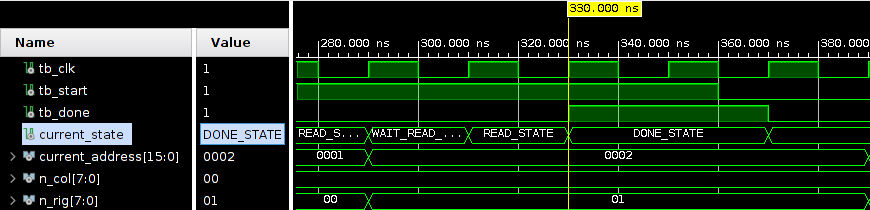
\includegraphics[width=\textwidth]{tb_no_image.png}
        \end{figure}

    \subsection{Reset asincrono}
    
        Vi è la possibilità che durante il regolare funzionamento della FSM, il segnale di \texttt{i\_rst} venga portato ad 1 con una tempistica non sincrona al segnale di clock.
        In questo caso il processo si risveglia e la FSM torna allo stato di \texttt{RESET}, indipendentemente dallo stato in cui si trova e dalle  azioni che sta svolgendo.
        
    
    \begin{figure}[h]
        \centering
        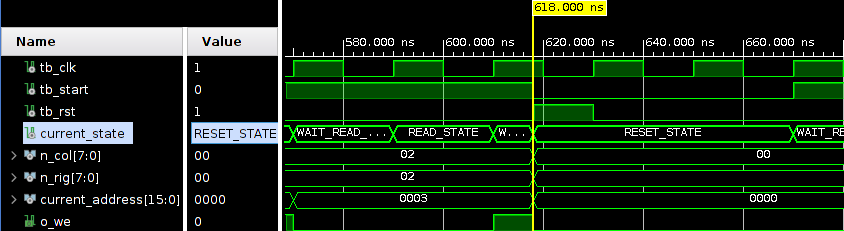
\includegraphics[width=\textwidth]{tb_async_reset.png}
    \end{figure}
    
    \subsection{Immagini di varie dimensioni}
    
        La FSM è stata inoltre sottoposta a più test che ne verificassero il funzionamento anche con dimensioni dell'immagine estreme come, ad esempio, 128x128 e 1x1 o con notevoli differenze tra il numero di righe ed il numero di colonne, per esempio 1x128.
        
    \subsection{Più immagini consecutive}
    
        Nel caso vi siano ulteriori immagini da equalizzare, sono stati creati dei test che verificassero il corretto funzionamento della FSM sia nel caso in cui avviene un reset tra un'immagine e l'altra, sia nel caso in cui questo non si verifica.
        
        \begin{figure}[h]
            \centering
            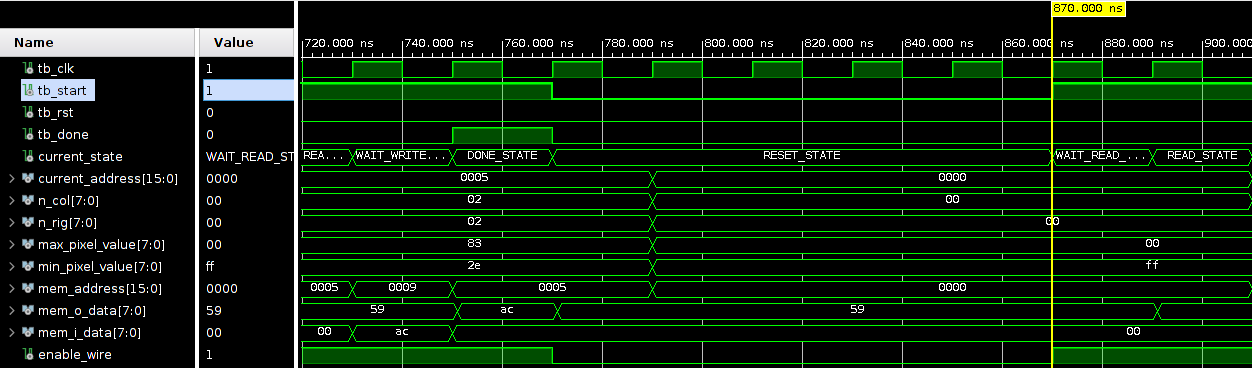
\includegraphics[width=\textwidth]{tb_multiple_no_reset.png}
        \end{figure}
        
    
    
    \subsection{Ricerca ottimizzata di massimo e minimo}
    
        Nel caso in cui, durante il riconoscimento dei valori di massimo e di minimo, si incontri un massimo di 255 e un minimo di 0 prima della lettura completa dei rimanenti byte, la FSM salta direttamente allo stato di \texttt{SHIFT COUNTER}.
    
        \begin{figure}[h]
            \centering
            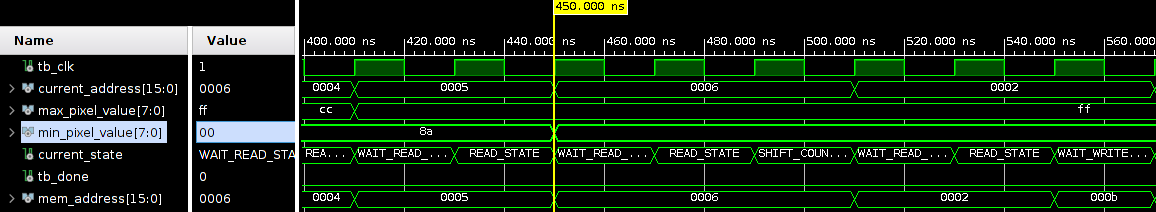
\includegraphics[width=\textwidth]{tb_fast_max_min.png}
        \end{figure}
        

\section{Conclusioni}

        In conclusione, lo sviluppo di questo progetto ha portato all'acquisizione e al consolidamento di conoscenze base sulla progettazione e sulla sintesi di componenti logici.
        Le conoscenze teoriche assimilate durante il corso sono state quindi applicate in un contesto pratico.
      


\end{document}